\section{Opsamling}
Da det må antages at fejl kan forkomne under transmissionen, skal pakkerne tilføjes en header og trailer, som kan kompensere for de fejl der måtte forvæntes at opstå under transmissionen. Denne redundante information er nødvendig for en pålidelig kommunikation, men dette optager plads for data som ellers kunne være sendt. Effektiviteten af den anvendte pakkeformat vil derfor kunne beregnes ved nedenstående formel: 

\begin{equation}
nyttevirkning = \frac{Data}{Headder + Data}
\label{eq:Nyttevirkning}
\end{equation}

Uafhængig af hvor meget data der der sendes af gangen fra det øverste lag vil den administrative data være af fast længde. På applikationslaget tilføjes en 32 bits header til hele beskeden. På datalinklaget tilføjes en header og trailer på i alt 44 bits, hvis der anvendes et CRC16 til fejldetektion. og yderligere 8 bits preample på det fysiske lag. Udover dette skal der tilføjes 52 bits for hver ACK der skal sendes tilbage igen. Hvis hver frame har en maksimal datalængde pakkelængde er på henholdsvist 25 og 250 bytes, kan en nyttevirkningen udregnes som funktion af pakkelængden ved brug af formel \eqref{eq:Nyttevirkning}.  

\begin{figure}[h]
\centering
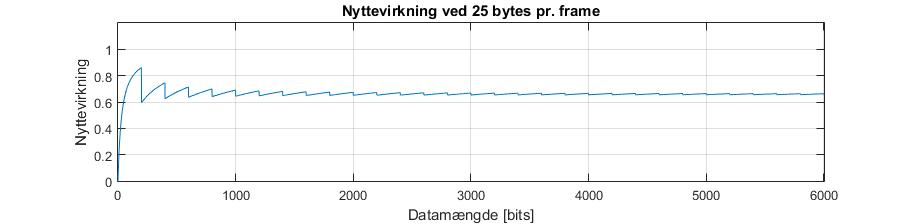
\includegraphics[scale=0.5]{Billeder/Nyttevirkning_25.jpg} 
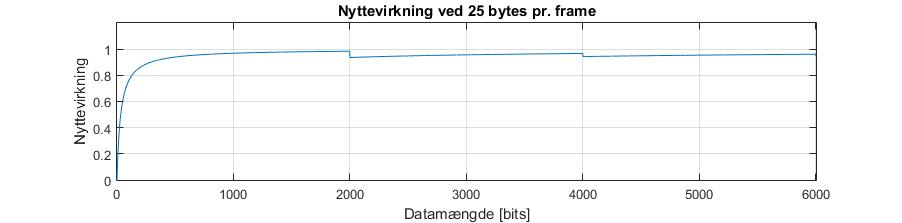
\includegraphics[scale=0.5]{Billeder/Nyttevirkning_250.jpg}
\caption{ Her ses hvordan nyttevirkningen af hver transmitterede tekstbesked, afhængeer af længden framelængden, og det total dataindhold som skal sendes fra applikationslaget}
\label{fig:Nyttevirkning_ved_25}
\end{figure}

Som vist af figur \ref{eq:Nyttevirkning}, har længden af datapakkerne en stor effekt på systemets nyttevirkning. Ved en pakkestørrelse på 25 bits + header, kan det aflæses af grafen at nyttevirkningen vil konvergere mod 65 \% efterhånden som længden af den sendte besked går mod uendelig. Tidobles indholdet af hver pakke så 

Det endelige Designklassediagram
